\documentclass[29pt,a4paper]{moderncv}

% moderncv themes
%\moderncvtheme[blue]{casual}                 % optional argument are 'blue' (default), 'orange', 'red', 'green', 'grey' and 'roman' (for roman fonts, instead of sans serif fonts)\textsl{}
\moderncvtheme[green]{banking}                % idem

\usepackage[T1]{fontenc}
% character encoding
\usepackage[utf8x]{inputenc}               	% replace by the encoding you are using
\usepackage[italian]{babel}
\usepackage{color}

% adjust the page margins
\usepackage[scale=0.8]{geometry}
\recomputelengths                          	% required when changes are made to page layout lengths

\fancyfoot{} % clear all footer fields
\fancyfoot[L,RO]{\thepage}           		% page number in "outer" position of footer line
\fancyfoot[R,LO]{\footnotesize} 			% other info in 

\begin{document}
\section{\textbf{Change History:}}
\begin{tabbing}
\\\textbf{Date:} ~~~~~~~~~~~~~~~~~\= \textbf{Version Update:}~~~~~~~~\= \textbf{Member:}~~~~~~~~~~~~~\= \textbf{Description:}\\
2013/08/22\> 1.0 \> fractals \> Document created.\\
2013/08/24 \> 1.1 \> fractals \>  Technical Requirements added\\
2013/08/24 \> 1.2 \> fractals \> Non-Functional Requirements added\\
2013/08/24 \> 1.3 \> fractals \>  Technical Specification added\\
2013/08/24 \> 1.4 \> fractals \> System Features added\\
2013/08/24 \> 1.5 \> fractals \> Use Cases added\\
2013/08/24 \> 1.6 \> fractals \> Entity Relationship Diagrams added.  \\
2013/08/24 \> 1.7 \> fractals \> Introduction added  \\
2013/08/24 \> 1.8 \> fractals \> Purpose added  \\
2013/08/24 \> 1.9 \> fractals \> Project Scope added  \\
2013/08/24 \> 2.0 \> fractals \> References added  \\
2013/08/24 \> 2.1 \> fractals \> System Description added  \\
2013/08/24 \> 2.2 \> fractals \> External Interface Requirements added  \\
2013/08/24 \> 2.3 \> fractals \> Open Issues added  \\
2013/08/24 \> 2.4 \> fractals \> Glossary added  \\
2013/08/24 \> 2.5 \> fractals \> Use Cases updated  \\
2013/08/24 \> 2.6 \> fractals \> Functional Requirements updated  \\
2013/08/24 \> 2.7 \> fractals \> Technical Requirements updated  \\
2013/08/24 \> 2.8 \> fractals \> Open Issues updated  \\
2013/08/24 \> 2.9 \> fractals \> Class Diagram added  \\
2013/08/24 \> 3.0 \> fractals \> Glossary updated  \\
2013/09/14 \> 2.9 \> Janine Venter \> Functional Features updated\\
2013/09/15 \> 3.0 \>  Janine Venter \> Technical Specification \\ \> \> \> updated\\
2013/09/15 \> 3.1 \> Janine Venter \> Project Scope updated\\
2013/09/15 \> 3.2 \>  Janine Venter \> System Description updated\\
2013/09/15 \> 3.3\> Janine Venter \> Support for Latex and \\ \> \> \> Mimetex libraries updated\\
2013/09/15 \> 3.4 \> Janine Venter \> Messaging updated\\
2013/09/15 \> 3.5 \>  Janine Venter \> Open Issues updated\\
2013/09/15 \> 3.6 \> Janine Venter \> Authorization updated\\
2013/09/15 \> 3.7 \> Janine Venter \> Scalability updated\\
2013/09/15 \> 3.8 \> Michelle Peens \> Entity Relationship Diagram updated\\
2013/09/15 \> 3.9 \> Janine Venter \> Use Cases updated\\
2013/09/15 \> 4.0 \> Stephan Botha \> Use case added for MimeTeX\\
2013/10/09 \> 4.1 \> Michelle Peens \> Updated the System Description\\
2013/10/09 \> 4.2 \> Michelle Peens \> Updated the Use Case Diagrams\\
2013/10/09 \> 4.3 \> Michelle Peens \> Updated the ERD diagram\\
2013/10/10 \> 4.4 \> Michelle Peens \> Updated the System Features\\
2013/10/10 \> 4.5 \> Michelle Peens \> Updated the Technical Requirements\\
2013/10/10 \> 4.6 \> Michelle Peens \> System Description: Register Added\\
2013/10/10 \> 4.8 \> Michelle Peens \> Project Scope Updated\\
2013/10/11 \> 4.9 \> Michelle Peens \> System Description: Support for LaTeX \\ \> \> \> and MimeTeX Libraries Updated\\
2013/10/11 \> 5.0 \> Michelle Peens \> System Description: Messaging \\ \> \> \> Updated\\
2013/10/11 \> 5.1 \> Michelle Peens \> System Description: Login \\ \> \> \> Updated\\
2013/10/11 \> 5.2 \> Michelle Peens \> Login API updated\\
2013/10/11 \> 5.3 \> Michelle Peens \> Message Sending API updated\\
2013/10/11 \> 5.4 \> Michelle Peens \> MimeTeX API updated\\
2013/10/11 \> 5.5 \> Michelle Peens \> Register User API Added\\
2013/10/11 \> 5.6 \> Michelle Peens \> Adding Deleting Contacts API \\ \> \> \> Added\\
2013/10/11 \> 5.7 \> Michelle Peens \> Data Clearing API Added\\
2013/10/11 \> 5.8 \> Michelle Peens \> Predefined Image Selection API \\ \> \> \> Added\\
2013/10/11 \> 5.9 \> Michelle Peens \> Security Features API Added\\
2013/10/11 \> 6.0 \> Michelle Peens \> Exit API Added\\
2013/10/11 \> 6.1 \> Janine Venter \> Updated Document Purpose\\
2013/10/12 \> 6.2 \> Janine Venter \> Project Scope Updated\\
2013/10/12 \> 6.3 \> Janine Venter \> System Description Updated\\
2013/10/12 \> 6.4 \> Janine Venter \> System Description: Support for LaTeX and \\ \> \> \> MimeTeX Libraries Updated\\
2013/10/12 \> 6.5 \> Janine Venter \> System Description: Messaging \\ \> \> \> Updated\\
2013/10/12 \> 6.6 \> Janine Venter \> System Description: Login Updated\\
2013/10/12 \> 6.7 \> Janine Venter \> Login API updated\\
2013/10/12 \> 6.8 \> Janine Venter \> Message Sending API Updated\\
2013/10/12 \> 6.9 \> Janine Venter \> MimeTeX API Updated\\
2013/10/12 \> 7.0 \> Janine Venter \> Predefined Image Selection API \\ \> \> \> Updated\\
2013/10/12 \> 7.1 \> Janine Venter \> External Interface Requirements \\ \> \> \> Updated\\
2013/10/12 \> 7.2 \> Janine Venter \> Authorization Updated \\
2013/10/12 \> 7.3 \> Janine Venter \> Scalability Updated \\
2013/10/12 \> 7.4 \> Michelle Peens \> Technical Specification Updated \\
2013/10/12 \> 7.5 \> Janine Venter \> Open Issues Updated \\
2013/10/12 \> 7.6 \> Janine Venter \> Added Diagram of each class\\
2013/10/12 \> 7.7 \> Janine Venter \> Updated Class diagram\\
2013/10/23 \> 7.8 \> Janine Venter \> Updated Class diagram\\

\end{tabbing}


\newpage
\section{\textbf{Table of Contents:}}
\begin{tabbing}
\\\textbf{Subject}: ~~~~~\= ~~~~~~~~~~~~~~~~~~~~~~~~~~~~~~~~~~~~~~~~~~~~~~~~~~~~~~~~~~~~~~~~~~~~~~~~~~~~~~~~~~~~~~~\= \textbf{Page}:
\\\newline
1. Introduction \> \> 4\\							
\> 1.1 Purpose 	\> 4\\							
\> 1.2 Document Conventions\> 4 					\\
\> 1.3 Project Scope \> 4							\\
\> 1.4 References \> 4						\\
2. System Description \> \> 5					\\
3. Functional Requirements \> \> 5\\				
\> 3.1 System Features \> 6\\
\> 3.2 Use Cases \> 7\\
\> 3.3 Class Diagram \> 10\\
\> 3.4 Entity Relationship Diagram \> 12\\
4. External Interface Requirements \> \> 13\\
5. Technical Requirements (Non-Functional) \> \> 14\\
\> 5.1 Non-Functional Requirements \> 14\\
\> 5.2 Technical Requirements \> 14\\
6. Open Issues \> \> 15			\\				
7. Glossary \> \> 16 			\\				

\end{tabbing}
\newpage
	%\maketitle
	%\vspace{-10mm}
	%Section
	\section*{\textbf{1. Introduction}}
	\vspace{4mm}
	
		\textbf{1.1 Purpose}
			\\This document serves as an agreement between our team of developers and our client Mr. Will van Heerden. This agreement covers the requirements for the mobile Latex chat application which will support users with their communication in a scientific and mathematical environment. This document will ensure that the requirements for this application is clear and agreed upon by all parties involved, and the development processes and phases to follow will be based on the requirements set out herein.\\
		\vspace{1mm}
		
		\noindent \textbf{1.2 Document Conventions}
			\begin{itemize}
				\item Document Formatting: LaTeX
				\item UML Diagrams: Diagram Designer, Visual Paradigm
			\end{itemize}
		\vspace{5mm}
		%Section
		
		\noindent \textbf{1.3 Project Scope}
			\\The aim of the project is to develop an open source android XMPP chat client which supports the embedded LaTeX base equations that can be rendered as images on the mobile device. LaTeX based equations will be rendered on the handset to produce mathematical equations. The system provides the ability to view (preview), edit and correct equations before sending.
			\parindent 5mm The application functionality will be similar to that of \textit{yaxim}. Exchange of text messages and images of mathematical expressions will be possible through our software solution. The TeXchat application will have the ability to show a preview of the entered mathematical equation, send that equation as LaTeX code to the receving client and then render it on their handset. 
			
		\vspace{5mm}
		
	\noindent \textbf{1.4 References}
		\begin{itemize}
		\item Mr. Will van Heerden.
		\item Android Authors, 2013. Android NDK.\\ {[Online]} Available at: http://developer.android.com/tools/sdk/ndk/index.html
			\\{[Accessed 18 August 2013].}
		\end{itemize}
		\vspace{5mm}
		
	%Section
\newpage
	\section*{\textbf{2. System Description}}
	\vspace{4mm}
		\noindent The goal of our software application is to provide a chat service that will allow users to exchange normal text messages and send mathematical equations displayed in a rendered image format.  The application is intended to provide a service to users that require the ability and support for a chat client that allows them to communicate more efficiently and effortlessly in a scientific, and mathematical context. It will provide a more usable mobile version of a Latex chat application.\\ 
		
		\noindent\textbf{Support for LaTeX and MimeTeX Libraries}
		\\The application makes use of a Latex based library (MimeTeX) for the the rendering of equations as images on the mobile device.  For this reason we have implemented the support for the MimeTex library, through the use of the Android NDK (Native Development Kit), which allows us to embed the native C/C++ code of the MimeTeX library, in the source code. 
		\parindent 5mm The NDK acts as a bridge between the C/C++ code and Java code. The library is compiled through Eclipse using a special makefile that sets the correct compiler flags to indicate that it is in math mode and not text mode. The compiler flags represent different capabilities of the MimeTeX library, in this case we set it to math mode to support the mathematical LaTeX equations.\\
		
		
		\noindent\textbf{Messaging}
		\\The purpose of this application is for messaging to be possible between multiple clients on the server. The application now supports this feature as well as allowing a user to send both plain text messages and Latex based equations, which are rendered on the client side and displayed as an inline images.
		\parindent 5mm The rendering of the Latex based equations on the client side is provided through the use of the Mimetex library. The messages sent between the various clients on the server is stored statically through making use of a client side SQLite database, which also provides the functionality for the retrieval of messages.
		\\Unsent messages, such as messages sent while the user was offline, is stored on the server and as soon as the client is online these messages are fetched and displayed on the user's handset. The server uses a queue to store these messages.\\
		
		\noindent\textbf{Login}
		\\The application allows a user to log in using an appropriate username and password combination. A user is authenticated by logging into the server.  If a username and password combination is invalid the server will automatically hinder the user from logging in. Our user authentication component is implemented by the functionality provided by the server. The user is informed by the application that his/her attempt to log in was unsuccessful.\\
		
		\noindent\textbf{Register}
		\\The application allows someone to register to the TexChat service as a new user. Through the user registration form the user provides the necessary information and selects a username and password combination that is later used to authenticate the user on the server. After a user is successfully registered, he can immediately log in and start using the messaging functionality provided.
		
	\vspace{5mm}
	
\newpage	
	%Section
	\section*{\textbf{3.Functional Requirements}}
	\vspace{4mm}
	\noindent \textbf{3.1 System Features}\\
	
		\noindent \textbf{Login API}
		\begin{itemize}
			\item Logging in is possible through a username and password combination which is authenticated by the server.
			\item Provides a remember me component, which can be enabled or disabled by the user, option to log you in automatically the next time you open the application.
			\item Option to logout at the user’s request.
			\\
		\end{itemize}
		
		\noindent \textbf{Viewing Contact List API}
			\begin{itemize}
				\item Shows all contacts available for a specific user on the server’s contact roster.
				\item Display’s each contact’s status, available or unavailable, and the contact name.
				\item A user also has the ability to interact with the contact list.  By clicking on a specific contact, the messaging activity is started, and all messages with that particular contact is diplayed.\\
			\end{itemize}
		
		\noindent \textbf{Message Sending API}
			\begin{itemize}
				\item Allows message sending between a user and his/her contacts available on the server, both online and offline.  
				\item Messaging between an online and an offline contact is achieved through a queuing system provided by the server.
				\item All messages should be displayed for a particular contact, including previous messages sent or received and thus be retrieved from a static database on the client side (the device).
				\item Message display is updated instantly on the android client, i.e as soon as a new message is received or sent the view is updated to reflect the action instantly.
				\\
			\end{itemize}
			
		\noindent \textbf{MimeTeX API}
			\begin{itemize}
				\item Rendering of mathematical equations on the android client.
				\item The ability to preview, edit and correct an equation created by a user is provided before the equation is sent to a particular client.
				\item Equation is placed inline with the normal text message to allow for the continuous editing of the text message itself.
				\item The equation sent or received should be rendered on the client side, i.e on the android device itself. This rendering of an equation to an image should be done on the client side when the equation is being previewed, sent or when an equation is received as part of a message.
				\item This API is used in the Message Sending API.
				\\
			\end{itemize}
			
		\noindent\textbf{Register User API}
			\begin{itemize}
				\item A first time user of the application is provided with the option of registering as a new user on the server.
				\item Once a user has successfuly registered, they should be able to login immediately and use the contacts and messaging features provided.
				\\
			\end{itemize}
			
		\noindent\textbf{Adding Deleting Contacts API}
			\begin{itemize}
				\item The application should allows a user to add and delete contacts on request.
				\item Once a user has been added to another clients contact list, the user is provided with the ability to accept or reject the new proposed contact. Thereby providing an invite based adding of contacts.
				\item Once a contact is deleted from a user’s contact list, all relevant messages is deleted and the contact removed.
				\\		
			\end{itemize}	
			
		\noindent\textbf{Data Clearing API}
			\begin{itemize}
				\item A user is provided with the option to delete and clear message data on request. Once a user has selected a particular contact and utilizes the delete chat option, all relevant messages, sent and received, is cleared from the database on the client side.
				\\		
			\end{itemize}	
			
		\noindent\textbf{Predefined Image Selection API}
			\begin{itemize}
				\item To make the application more user friendly, it allows easy selection of predefined equations and functions (in image format) that a user can click on, to mitigate the tedious construction of equations using the Latex based syntax.
				\\		
			\end{itemize}
			
		\noindent\textbf{Security Features API}
			\begin{itemize}
				\item Once a user logs into the application, all sensitive user information, i.e username and password is encrypted and saved statically in the database on the client side.  This saving of sensitive data is required for features such as the remember me component.
				\\		
			\end{itemize}
		
		\noindent\textbf{Exit API}
			\begin{itemize}
				\item The application should provide the user with an option to exit and close the application. When this feature is utilized, the connection with the server is terminated, and the user is effectively logged out and offline.
				\\		
			\end{itemize}
			
	\noindent \left\textbf{3.2 Use Cases: }\\
	\vspace{4mm}
		\\ \noindent \left\textbf{Login}\\
		\\ \begin{figure*}
					\centering
					\\ 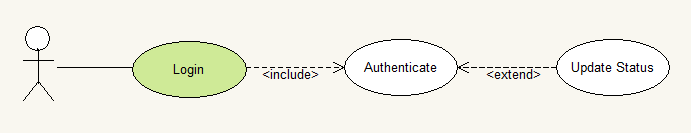
\includegraphics[width=6.0in, height=1.2in]{./loginCase.png}
					\\\caption{[Figure 1] Login Use Case}
			\end{figure*}\\
			
		\\ \noindent \left\textbf{Logout}\\
			\\ \begin{figure*}
						\centering
						\\ 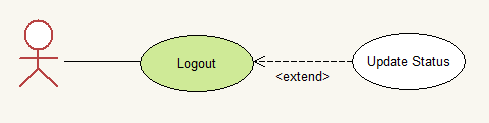
\includegraphics[width=6.0in, height=1.2in]{./ucLogout.png}
						\\\caption{[Figure 2] Logout Use Case}
				\end{figure*}\\
\newpage				
		\noindent \left\textbf{View Contact List}\\
		\begin{figure*}
					\centering
					\\ 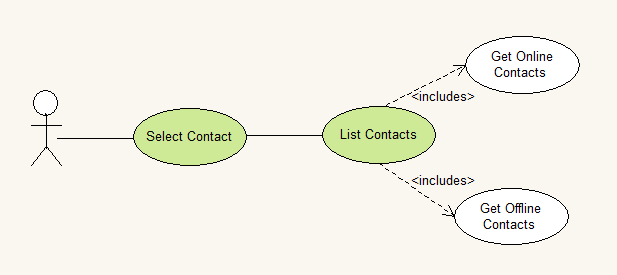
\includegraphics[width=6.0in, height=3.2in]{./viewContactsCase.png} \\
					\\\caption{[Figure 3] View Contact List Use Case} \\
		\end{figure*}\\ 
				
		\noindent \left\textbf{Messaging}\\
		\begin{figure*}
			\centering
			\\ 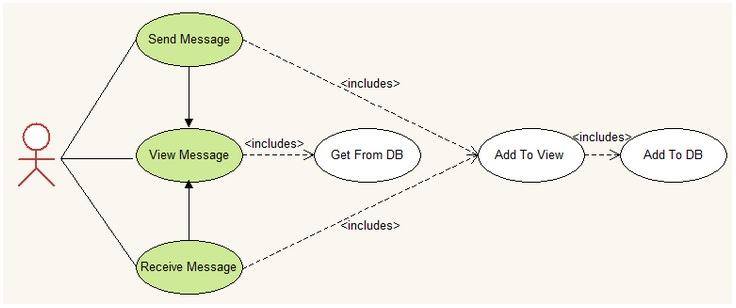
\includegraphics[width=6.0in, height=3in]{./messagingUseCase.jpg}
			\\\caption{[Figure 4] Messaging Use Case}\\
		\end{figure*}
\newpage		
		\noindent \left\textbf{Exit}\\
		\begin{figure*}
			\centering
			\\ 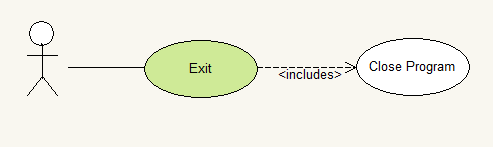
\includegraphics[width=6.0in, height=1.5in]{./exitCase.png}
			\\\caption{[Figure 5] Exit Use Case}\\
		\end{figure*}
		
	
		\noindent \left\textbf{MimeTeX}\\
		\begin{figure*}
			\centering
			\\ 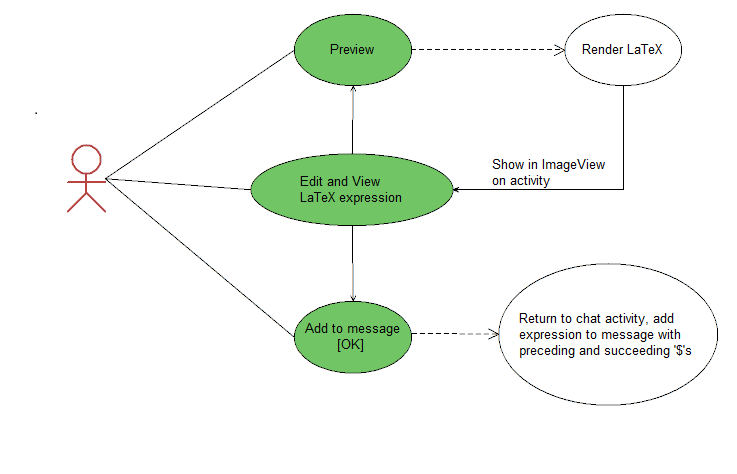
\includegraphics[width=6.0in, height=3.0in]{./MimeTeXUseCase.png}
			\\\caption{[Figure 5] MimeTeX Use Case}\\
		\end{figure*}
		
\newpage	
	\noindent \\ \left\textbf{3.3 Class Diagrams}\\
			\begin{figure*}
				\centering
				\\ 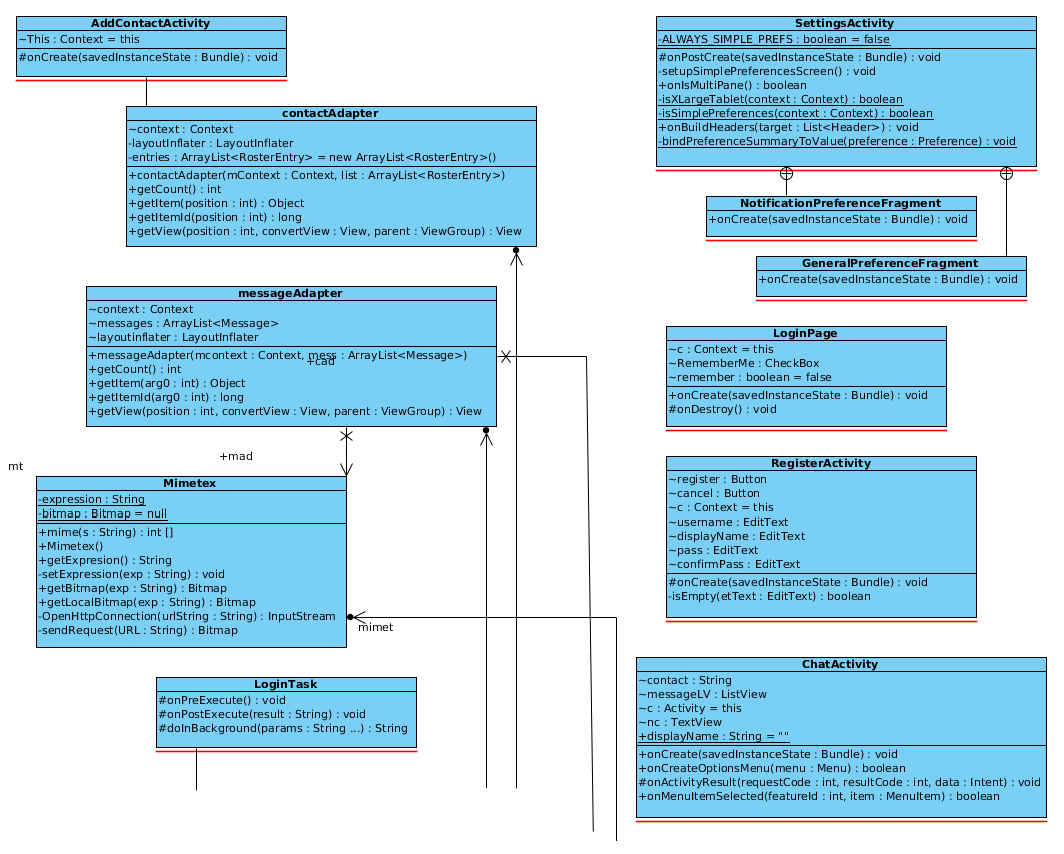
\includegraphics[width=6.7in, height=7.5in]{./classDiagram_part1.jpg}
				\\\caption{[Figure 6] Class Diagram}\\
			\end{figure*}
			

\begin{figure*}
				\centering
				\\ 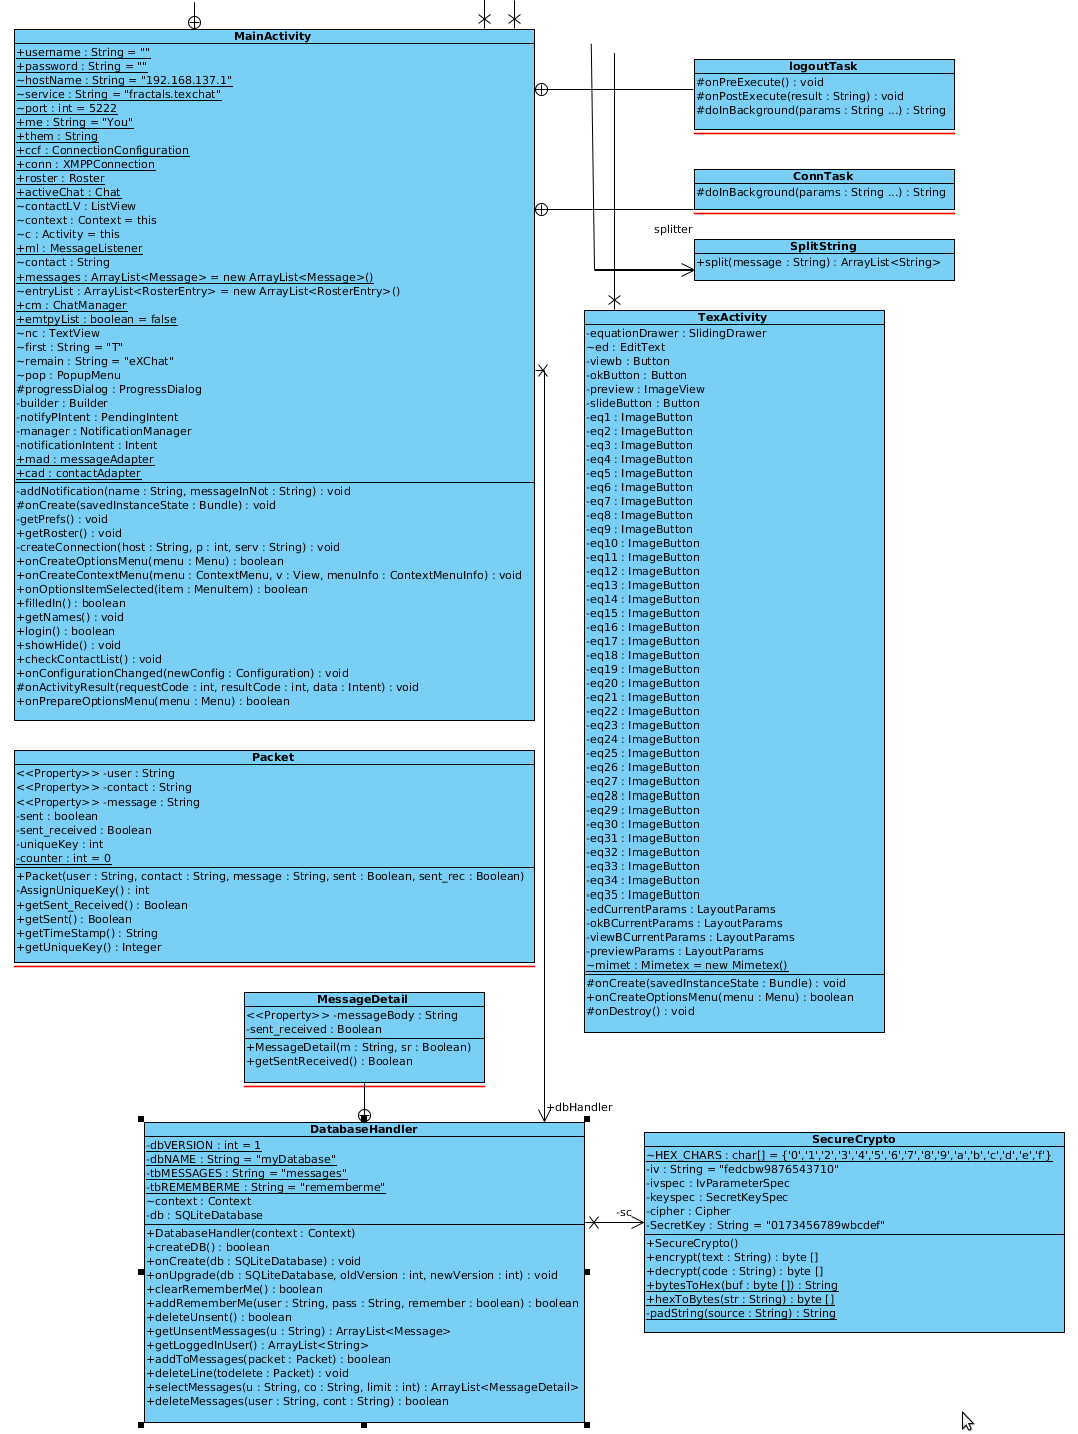
\includegraphics[width=6.7in, height=8.6in]{./classDiagram_part2.jpg}
				\\\caption{[Figure 6] Class Diagram Continued}\\
			\end{figure*}
\newpage	
	\\ \noindent \textbf{3.4 Entity Relationship Diagram}
	\\The system makes use of an SQLite database on the client side. This database contains two tables, namely Messages and Rememberme that is used to record message histories for a particular client as well as to remember the logged in user if applicable. 
	\parindent 5mm The database cleanup functionality is included and utilized at the user’s request through a delete message history option. When a user utilizes this option, all data with regard to a particular contact will be removed and cleared from the client side database.
	\\ \\
	
	\begin{figure*}
		\centering
		\\ 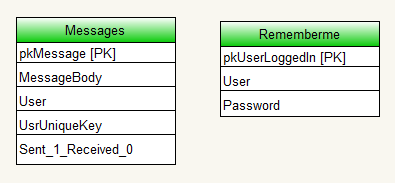
\includegraphics[width=4.5in, height=2.0in]{./erd.png}
		\\\caption{[Figure 7] ERD}\\
	\end{figure*}
	
\newpage	
	\section*{\textbf{4. External Interface Requirements}}
	\vspace{4mm}
		\begin{itemize}
			\item There is an external interface with the smack library.
			\item The mimeTeX library is also an external interface used within the application, the Native Development Kit acts as a bridge between Java and C/C++ when this library is used.
			\item The internal API uses the smack api to exchange the messages.
			\item The internal API's supply different functionality to the application.
			\item The internal API is used to store data in the database on the device.
		\end{itemize}

\newpage	
		\section*{\textbf{5. Technical Requirements(Non-Functional)}}
		\vspace{4mm}
		\noindent \textbf{5.1 Non-Functional Requirements}\\
		
		\noindent \textbf{Authentication}\\
			Authentication happens server side. \\
			A login page is created to allow the user access to the application and its features. \\
			As soon as the user’s credentials has been authenticated he/she is logged into the application.\\
			If their credentials do not match the available credentials on the server, the user is told that the login falied.\\
			
		\noindent \textbf{Authorization}\\
		The authorization is completed by checking whether the user is one of the users registered on the server and it allows them normal user privileges.
		These privileges entail the following: \\
		\begin{itemize}
		\item sending and receiving text messages
		\item sending and receving mathematical equations 
		\item deleting contacts
		\item adding contacts 
		\item deleting chat history
		\item logging out of the system
		\item changing the preferred server name and host.
		\\
		\end{itemize}
		
		\noindent \textbf{Scalability}\\
		At this point in time the system is developed to handle only 2 users at a time. It has not yet been tested with more than 2 active users at a time.
		\\It will later be scaled upwards to handle a larger amount of concurrent users. A solution to the scalability is by using an online server that will handle more than two clients concurrently\\
		
		
		\noindent \textbf{Audit-ability}\\
		The messages are logged on the phone’s database created by the application as soon as it is installed.\\
		
		\noindent \textbf{5.2 Technical Specification}\\
		Platforms to be supported:
		\begin{itemize}
			\item Android
			\\
		\end{itemize}
		The application is developed using Java and C/C++ programming languages.  The C/C++ languages are implemented as native code through the use of the Android NDK (Native Development Kit).
		The application is further developed to communicate both with a locally set up Jabber server, such as Openfire, as well as with a publicly available Jabber server through an internet connection.
		Lastly, the client side database used throughout is implemented in SQLite.
		\\
		
\newpage	
	\section*{\textbf{6. Open Issues}}
	\vspace{4mm}
		\begin{itemize}
			\item Visual elements and styling
		\end{itemize}
	\vspace{5mm}

\newpage	
	\section*{\textbf{7. Glossary}}
	\vspace{4mm}
		\begin{itemize}
			\item SDK - Software Development Kit
			\item NDK - Native Development Kit
			\item ADT - Android Development Toolkit plugin
			\item IDE - Integrated Development Environment
			\item RUP - Rational Unified Process
			\item XML - eXtensible Markup Language
			\item Agile - Development methodology
			\item MVC - Model View Controller
			\item UML - Unified Modelling Language
			\item API - Application Programming Interface
			\item MimeTex - LaTeX library ported to Android
			\item C - Programming language.
			
		\end{itemize}
	\vspace{5mm}
\end{document}